\documentclass[12pt,english]{article}
%%% PREAMBLE

%%% Install missing packages %%%
% tinytex::parse_install("MainText.log")

% Sometimes you have to run: tinytex::install_tinytex()
% and maybe: tlmgr_update()

\usepackage{bbding} % for checkmark symbol
\usepackage{booktabs}
%\usepackage{chngcntr} % Allows table and figure counters to be reset in Appendix
\usepackage[font=small,format=hang,justification=raggedright,labelfont=up,labelsep=space,singlelinecheck=false]{caption}
\usepackage{color} % use to color text
\usepackage[T1]{fontenc}
\usepackage{geometry} % set margins and stuff
\usepackage{graphicx}
\usepackage{lineno}
\usepackage{longtable}
\usepackage{microtype}
\usepackage{pdflscape} % Causes pages that are in landscape format to be rotated when viewing the pdf but print as usual
\usepackage{scrextend} % Allows you to change margins for section of text
\usepackage{setspace}
\usepackage{siunitx}
\usepackage{titlesec}
\usepackage[dvipsnames]{xcolor} % use to get more colors

%\DisableLigatures{encoding = *, family = *}
\DisableLigatures[f]{encoding = *, family = *} %% <- only disables f-ligatures

\PassOptionsToPackage{hyphens}{url}\usepackage[hidelinks]{hyperref} % enables hyperlinks
\urlstyle{same} % Maintains URLs in the same font as the rest of the text

% Bibliography related
\usepackage{natbib}                            % For citations
\bibpunct{(}{)}{;}{a}{}{;}
\setlength{\bibhang}{2em}

%\addbibresource{KlibanskyFishResearch_1.5}
%\graphicspath{ {images/} }
\geometry{verbose,letterpaper,tmargin=2.54cm,bmargin=2.54cm,lmargin=2.54cm,rmargin=2.54cm}
%\linenumbers

\captionsetup{figurename=Fig.}

% Define heading formatting
\titleformat{\section}
   {\small\mdseries\scshape}{\thesection}{1em}{}

\titleformat{\subsection}
   {\small\mdseries\itshape}{\thesubsection}{1em}{}

%%% Main document
% BEGIN DOCUMENT
\usepackage{Sweave}
\begin{document}
\Sconcordance{concordance:MainText.tex:MainText.Rnw:%
1 56 1 1 0 2 1 1 9 1 11 1 5 1 14 273 1}







% Top matter
\title{Evaluating procedures for updating catch advice between stock assessments of reef fishes with management strategy evaluation}
\author{Nikolai Klibansky,  Shannon Calay, Rob Cheshire,\\
Cassidy Peterson, Kyle Shertzer, Erik Williams, and Matt Vincent\\\\
Southeast Fisheries Science Center, \\
National Marine Fisheries Service, NOAA,\\
101 Pivers Island Road, Beaufort, North Carolina, 28516, USA}
\maketitle

\begin{abstract}
We built operating models for three reef fish species from the US Southeast Atlantic, based on recent stock assessments. We developed 10 scenerios and 13 management procedures. Management procedures varied in terms of how often stock assessments were conducted, and how catch advice was adjusted between stock assessments.

\end{abstract}

\begin{flushleft}
\begin{spacing}{1.9}
\setlength{\parindent}{1cm} % Indent paragraphs after the first one

\section*{Introduction}
We can only do stock assessments every few years. It would be nice to know if there were ways that we could adjust catch advice between stock assessments to improve.


\section*{Materials and Methods}
We used the most recent stock assessments from US Southeast US Atlantic for Red Porgy, Black Sea Bass, and Vermilion Snapper.

\subsection{Evaluating management procedures}

\section*{Results}


\section*{Discussion}

Some broad conclusions

Which factors seem to account for the most variation in results in general?
\begin{itemize}
\item Above all, results differ between operating models (i.e. species)
\item Scenario is the next most important factor, particularly depletion scenarios and regime change
\end{itemize}

\section*{Acknowledgements}
We thank everyone.

\end{spacing}
\end{flushleft}

% \printbibliography
%%% LITERATURE CITED %%%
%\printbibliography
\clearpage
\section*{Literature Cited}
\renewcommand{\refname}{}
\bibliographystyle{ecosphere} % Modified from ecology.bst
\vspace{-1cm}

\bibliography{KlibanskyFishResearch_1.5}


%% TABLES
\newpage
\section*{Tables}

%\input{../Results/biodivByArea.tex}
%\clearpage


%% FIGURES %%
\newpage
\section*{Figures}

\begin{figure}[!ht]
\begin{center}
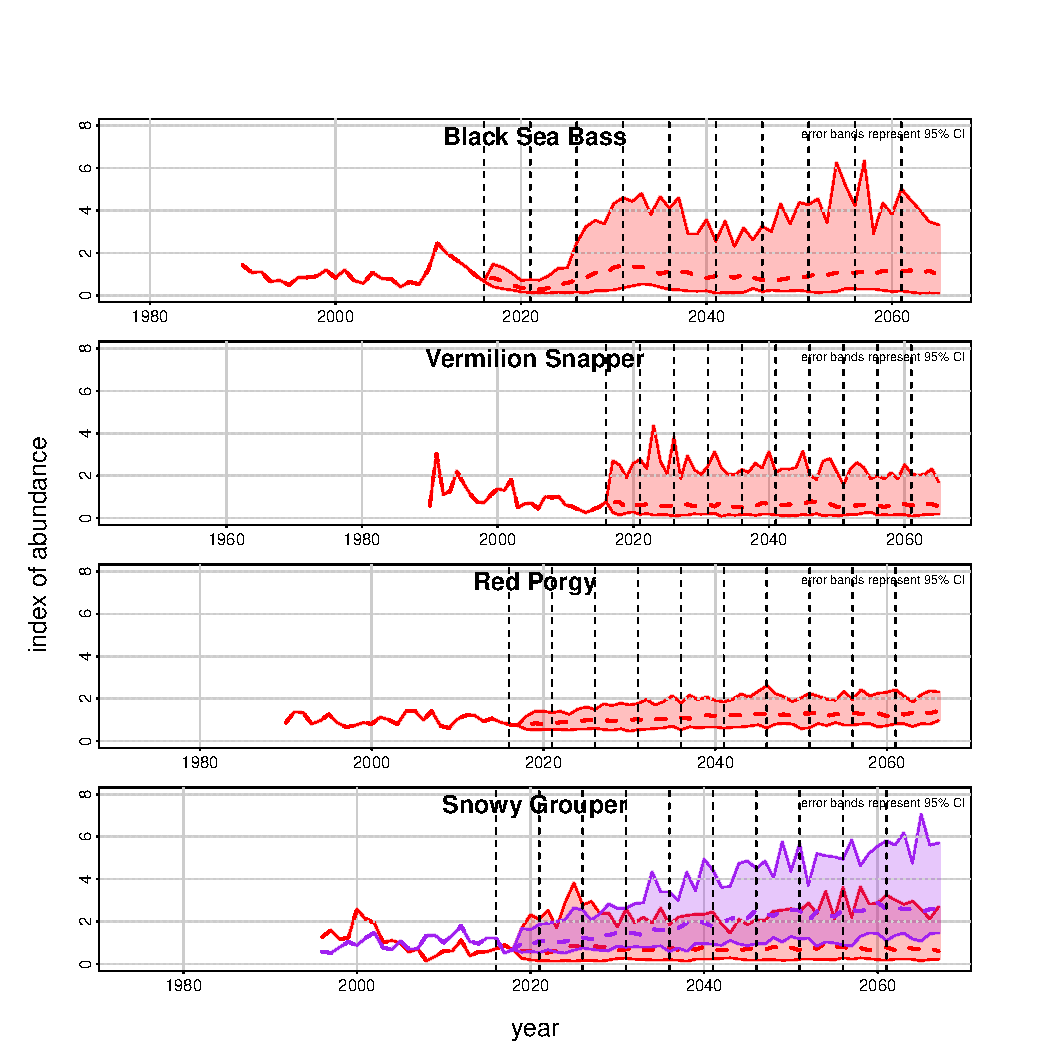
\includegraphics[width=6in,height=7in]{../Figs/AddInd.pdf}
\end{center}
\begin{flushleft}
\caption{Indices derived from BAM stock assessments available during the projection period, for the SCA\_5 MP in the Base scenario. Shaded areas represent 95\% CI for indices among simulation runs.}
\label{fig:phasePlot1}
\end{flushleft}
\end{figure}


\begin{figure}[!ht]
\begin{center}
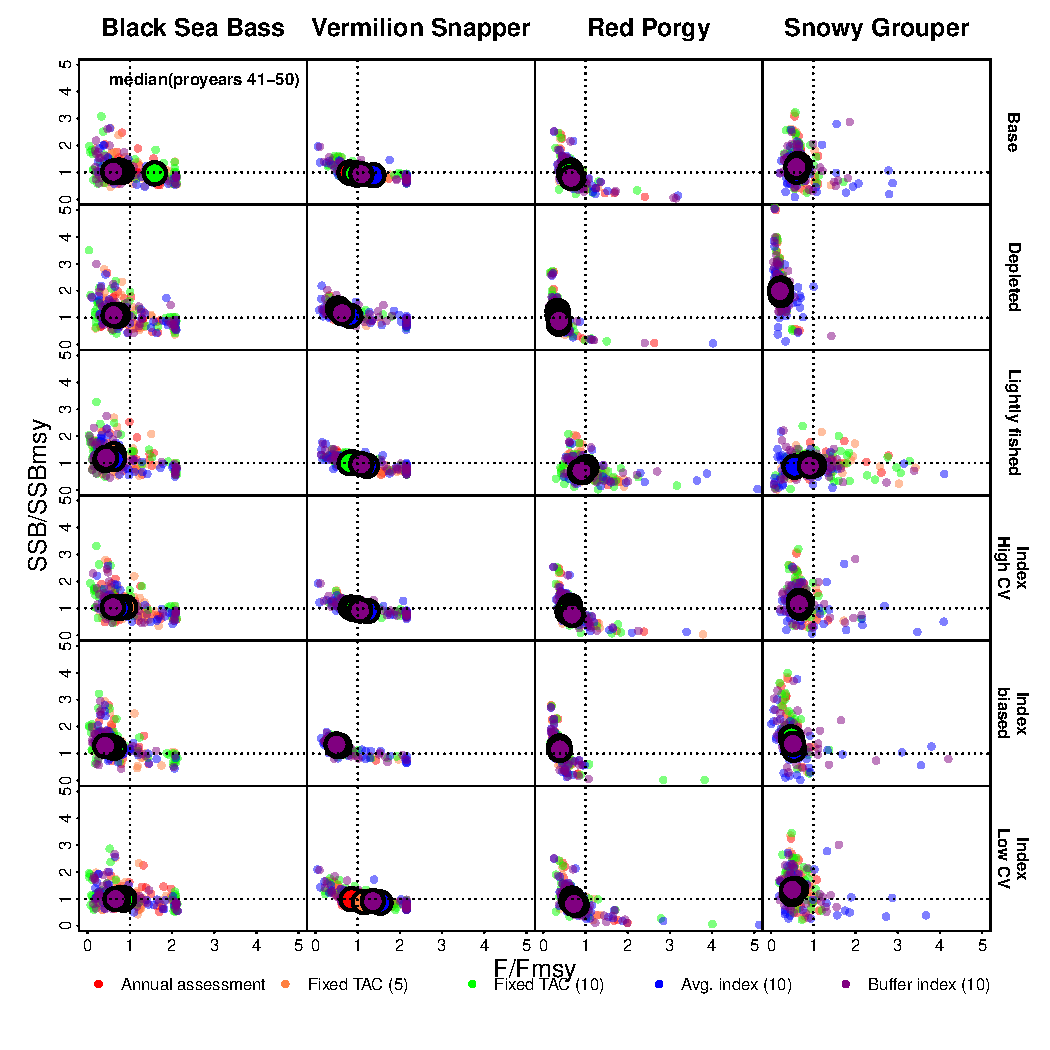
\includegraphics[width=6in,height=7in]{../Figs/phasePlot1.pdf}
\end{center}
\begin{flushleft}
\caption{Phase plots for the base scenario and the first set of experimental scenarios}
\label{fig:phasePlot1}
\end{flushleft}
\end{figure}

% \begin{figure}[!ht]
% \begin{center}
% 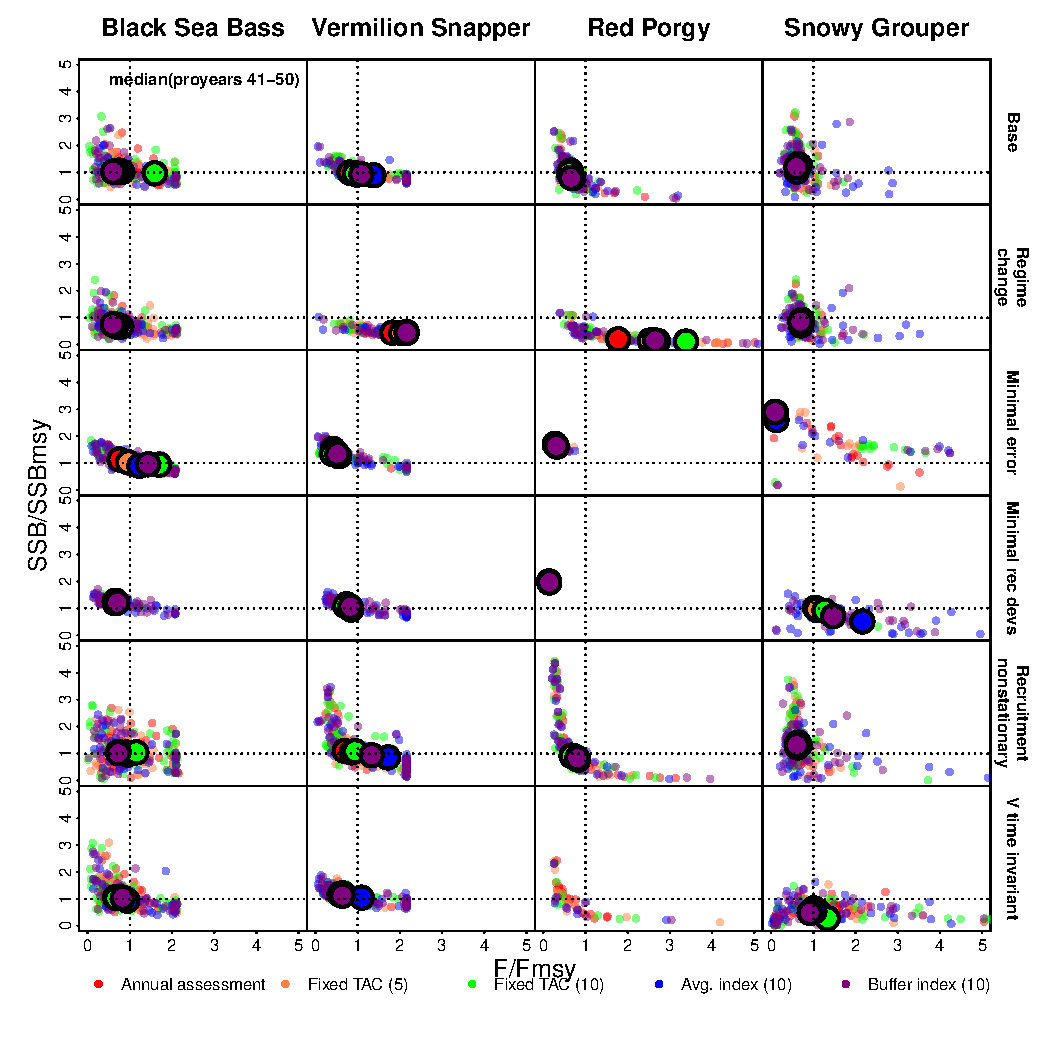
\includegraphics[width=6in,height=7in]{../Figs/phasePlot2.pdf}
% \end{center}
% \begin{flushleft}
% \caption{Phase plots for the base scenario and the second set of experimental scenarios}
% \label{fig:phasePlot2}
% \end{flushleft}
% \end{figure}


%% APPENDIX
% \begin{appendix}
%
% \clearpage
% \section*{Appendix S1}
%
% \setcounter{table}{0}
% \renewcommand{\thetable}{S\arabic{table}}
%
% \input{../Results/Appendix.tex}
%
% \input{../Results/biodivByBlock.tex}
%
% \end{appendix}


% END DOCUMENT
\end{document}
